%
% This work is licensed under a Creative Commons Attribution-ShareAlike 4.0 International License.
% http://creativecommons.org/licenses/by-sa/4.0/
%

% DO NOT COMPILE THIS FILE DIRECTLY!
% This is included by the other .tex files.


\begin{frame}
    
\includegraphics[scale=.3]{images/logo-circl-Forensics.png}
    \begin{itemize}
        \item[]
        \item[]
        \item[] 3. Other Sources of Information
    \end{itemize}
\end{frame}


\begin{frame}[fragile]
  \frametitle{3.1 Recycle Bin - User support to undelete}
    \begin{itemize}
        \item Files move to Recycle Bin:
            \begin{itemize}
                \item Moved by mouse
		\item Right click: \texttt{Delete}
            \end{itemize}
        \item Not move to Recycle Bin:
            \begin{itemize}
		    \item Right click: \texttt{Delete + SHIFT}
		    \item Command line: \texttt{del}
		\item Files on network shares
            \end{itemize}
        \item NukeOnDelete
            \begin{itemize}
		    \item \texttt{HKEY\_USERS/\_UUID\_/Software/Microsoft/Windows/CurrentVers}
		    \item[]\texttt{ion/Explorer/BitBucket/Volume/\{\_Volume ID\_\}/NukeOnDelete}
                    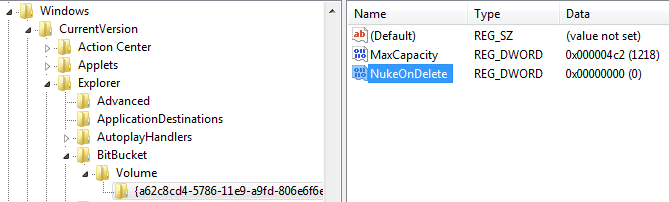
\includegraphics[scale=.3]{images/nukeOD.png}
            \end{itemize}
    \end{itemize}
\end{frame}


\begin{frame}[fragile]
  \frametitle{3.1 Recycle Bin - Life-Investigate}
    \begin{itemize}
        \item Play script: \texttt{TextFile.txt} 
            \begin{itemize}
		\item 2019-04-30 17:31:57 UTC+2:  Born
		\item 2019-04-30 17:34:44 UTC+2:  Content Modified
		\item 2019-04-30 17:35:32 UTC+2:  Deleted
		\item[]
            \end{itemize}
        \item Analyze Recycle.Bin:
        \item[] 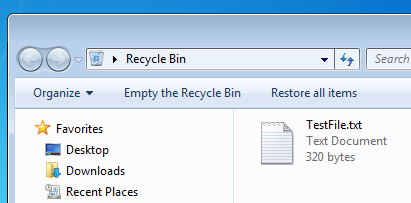
\includegraphics[scale=.45]{images/f15_recycle.png}
    \end{itemize}
\end{frame}


\begin{frame}[fragile]
  \frametitle{3.1 Recycle Bin - Forensics}
    \begin{itemize}
        \item Play script: \texttt{TextFile.txt} 
            \begin{itemize}
		\item 2019-04-30 17:31:57 UTC+2:  Born
		\item 2019-04-30 17:34:44 UTC+2:  Content Modified
		\item 2019-04-30 17:35:32 UTC+2:  Deleted
		\item[]
            \end{itemize}
        \item Analyze \texttt{Recycle.Bin} directory:
  \begin{lstlisting}[basicstyle=\tiny]
/$Recycle.Bin/S-1-5-21-3408732720-2018246097-660081352-1000/
	129 Apr  5 11:46  desktop.ini
	544 Apr 30 17:35 '$IOMHI9A.txt'
	320 Apr 30 17:34 '$ROMHI9A.txt'

strings \$ROMHI9A.txt 
		Test File
		=========
	This is a test file. It is just created to test Forensic
	Artifacts for the 'Recycle Bin'.
	.....

strings -el \$IOMHI9A.txt 
	C:\Users\John\Documents\recycleTest\TestFile.txt
  \end{lstlisting}
    \end{itemize}
\end{frame}


\begin{frame}[fragile]
  \frametitle{3.1 Recycle Bin - Forensics}
    \begin{itemize}
        \item Play script: \texttt{TextFile.txt} 
            \begin{itemize}
		\item 2019-04-30 17:31:57 UTC+2:  Born
		\item 2019-04-30 17:34:44 UTC+2:  Content Modified
		\item 2019-04-30 17:35:32 UTC+2:  Deleted
		\item[]
            \end{itemize}
        \item Analyze \texttt{Recycle.Bin} directory:
  \begin{lstlisting}[basicstyle=\tiny]
Fri Apr 05 2019 11:46:49
     328 m.c.      57-144-1 /$Recycle.Bin
     376 ...b    9632-144-1 /$Recycle.Bin/S-1-5-21- ..... -1000
     129 m.cb    9634-128-1 /$Recycle.Bin/S-1-5-21- ..... -1000/desktop.ini

Tue Apr 30 2019 17:31:57
     320 ...b   47164-128-1 /$Recycle.Bin/S-1-5-21- ..... -1000/$ROMHI9A.txt

Tue Apr 30 2019 17:34:44
     320 ma..   47164-128-1 /$Recycle.Bin/S-1-5-21- ..... -1000/$ROMHI9A.txt

Tue Apr 30 2019 17:35:32
     544 macb   44155-128-1 /$Recycle.Bin/S-1-5-21- ..... -1000/$IOMHI9A.txt
      48 mac.   47022-144-1 /Users/John/Documents/recycleTest
     320 ..c.   47164-128-1 /$Recycle.Bin/S-1-5-21- ..... -1000/$ROMHI9A.txt
     376 mac.    9632-144-1 /$Recycle.Bin/S-1-5-21- ..... -1000
  \end{lstlisting}
    \end{itemize}
\end{frame}


\begin{frame}[fragile]
  \frametitle{3.1 Recycle Bin - Exercise}
    \begin{itemize}
	    \item[] Invetigate extension of an index file \texttt{\$I.....} for binary file:
    \end{itemize}
    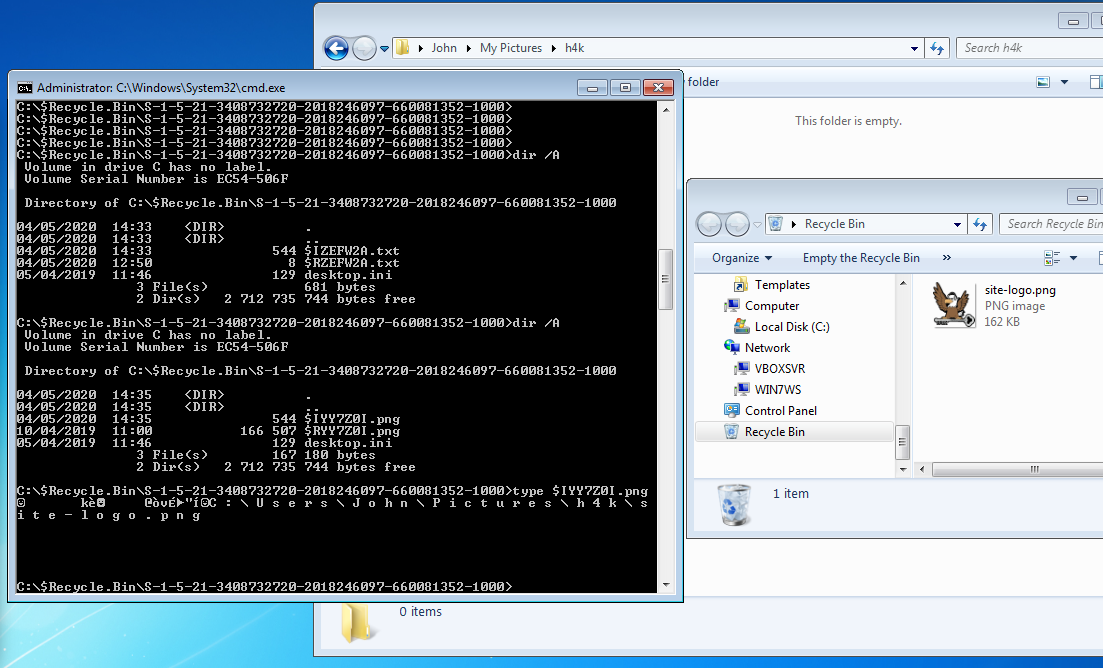
\includegraphics[scale=.27]{images/recycleEx.png}
\end{frame}


\begin{frame}[fragile]
  \frametitle{3.2 LNK Files}
    \begin{itemize}
        \item Provide information about files accessed
        \begin{itemize}
            \item Local
            \item Network shares
            \item Appached devices
        \end{itemize}
    \end{itemize}
  \begin{lstlisting}[basicstyle=\tiny]
Thu May 02 2019 14:54:02
     280 ...b       43701-144-1 /Users/John/Documents/prefetchTest
  
Thu May 02 2019 14:54:28
      66 macb       43702-128-1 /Users/John/Documents/prefetchTest/
      				PreFetchTest.txt
    2779 macb       43716-128-4 /Users/John/AppData/Roaming/Microsoft/
    				Windows/Recent/PreFetchTest.txt.lnk
    1573 macb       43922-128-4 /Users/John/AppData/Roaming/Microsoft/
    				Windows/Recent/prefetchTest.lnk
  \end{lstlisting}
\end{frame}


\begin{frame}[fragile]
  \frametitle{3.2 LNK Files}
    \begin{itemize}
        \item Provide information about files accessed
        \begin{itemize}
            \item Local
            \item Network shares
            \item Appached devices
        \end{itemize}
    \end{itemize}
  \begin{lstlisting}[basicstyle=\tiny]
exiftool PreFetchTest.txt.lnk

	...
	Create Date         : 2019:05:02 14:54:28+02:00
	Access Date         : 2019:05:02 14:54:28+02:00
	Modify Date         : 2019:05:02 14:54:28+02:00
	Target File Size    : 66
	Icon Index          : (none)
	Run Window          : Normal
	Hot Key             : (none)
	Drive Type          : Fixed Disk
	Volume Label        :
	Local Base Path     : C:\Users\John\Documents\prefetchTest\
				PreFetchTest.txt
	...
  \end{lstlisting}
\end{frame}


\begin{frame}[fragile]
  \frametitle{3.3 XP Restore Points}
    \begin{itemize}
        \item Backup of:
        \begin{itemize}
	    \item Critical system files
	    \item Registry partially
            \item Local user profiles
            \item But NO user data!
        \end{itemize}
        \item Created automatically:
        \begin{itemize}
            \item Every 24 hours
            \item Windows Update
	    \item Installation of applications incl. driver
            \item Manually
        \end{itemize}
        \item For user: Useful to recover a broken system
        \item For analyst:
        \begin{itemize}
	    \item \texttt{rp.log}
            \item Description of the cause
            \item Time stamp
            \item State of the system at different times
        \end{itemize}
    \end{itemize}
\end{frame}


\begin{frame}[fragile]
  \frametitle{3.4 VSS - Volume Shadow Copy Service}
    \begin{itemize}
	    \item Backup Service
            \begin{itemize}
	         \item System files
	         \item User data files
	         \item Operates on block level
            \end{itemize}
	    \item On live system
            \begin{itemize}
	         \item Run CMD as administrator
  \begin{lstlisting}[basicstyle=\tiny]
>vssadmin list shadows /for=c:/
vssadmin 1.1 - Volume Shadow Copy Service administrative command-line tool
(C) Copyright 2001-2005 Microsoft Corp.

Contents of shadow copy set ID: {33eb3a7b-6d03-4045-aa70-37b714d49c72}
   Contained 1 shadow copies at creation time: 10/04/2019 16:06:30
      Shadow Copy ID: {34d9910b-ac1d-4b10-b282-89dde217d0fb}
         Original Volume: (C:)\\?\Volume{a62c8cd4-5786-11e9-a9fd-806e6f6e6963}\
         Shadow Copy Volume: \\?\GLOBALROOT\Device\HarddiskVolumeShadowCopy1
         Originating Machine: Win7WS
         Service Machine: Win7WS
         Provider: 'Microsoft Software Shadow Copy provider 1.0'
         Type: ClientAccessibleWriters
         Attributes: Persistent, Client-accessible, No auto release, Differential,
	 Auto recovered
  \end{lstlisting}
            \end{itemize}
  \end{itemize}
\end{frame}


\begin{frame}[fragile]
  \frametitle{3.4 VSS - Configuration}
	    \begin{itemize}
		    \item[] \scriptsize{\texttt{HKEY\_LOCAL\_MACHINE/SYSTEM/CurrentControlSet/services/VSS}}
		    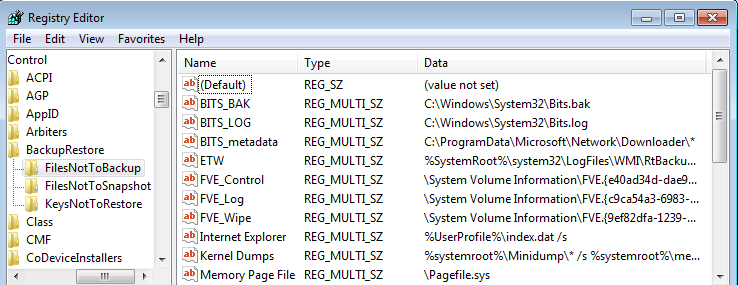
\includegraphics[scale=.3]{images/VSSConfig2.png}
		    \item[]
	    \item[] \scriptsize{\texttt{HKEY\_LOCAL\_MACHINE/SYSTEM/CurrentControlSet/Control/BackupRestore}}
		    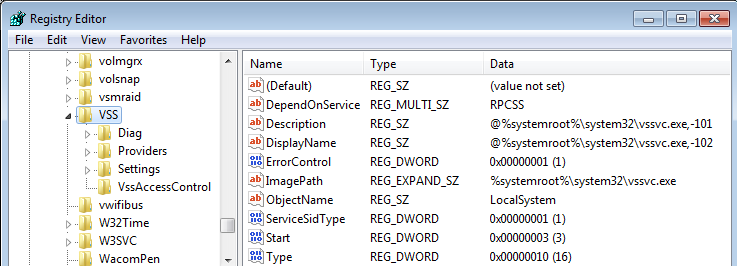
\includegraphics[scale=.3]{images/VSSConfig.png}
            \end{itemize}
\end{frame}


\begin{frame}[fragile]
  \frametitle{3.4 VSS - Analysis}
    \begin{itemize}
	    \item[] Analyze disk image
  \begin{lstlisting}[basicstyle=\tiny]
vshadowinfo -o $((512*206848)) 8d34ce.raw 

    Volume Shadow Snapshot information:
	Number of stores:	1

    Store: 1
	Identifier		: 237c8de3-5b99-11e9-9925-080027062798
	Shadow copy set ID	: 33eb3a7b-6d03-4045-aa70-37b714d49c72
	Creation time		: Apr 10, 2019 14:06:30.365699200 UTC
	Shadow copy ID		: 34d9910b-ac1d-4b10-b282-89dde217d0fb
	Volume size		: 11 GiB (12777947136 bytes)
	Attribute flags		: 0x0042000d
  \end{lstlisting}
	    \item[] Mounting VSC: A 2 step approach
  \begin{lstlisting}[basicstyle=\tiny]
sudo vshadowmount -o $((512*206848)) 8d34ce.raw /mount/vss/

sudo ls -l /mount/vss/
	-r--r--r-- 1 root root 12777947136 Jan  1  1970 vss1

sudo file /mount/vss/vss1
	/mount/vss/vss1: DOS/MBR boot sector, code offset 0x52+2, OEM-ID "NTFS 

sudo mount -o ro /mount/vss/vss1 /mnt/
  \end{lstlisting}
  \end{itemize}
\end{frame}


\begin{frame}[fragile]
  \frametitle{3.5 Prefetch Files \& SuperFetch}
    \begin{itemize}
        \item Boot prefetching for all Windows
	\item Application prefetching since XP
        \begin{itemize}
            \item Monitor an application when it starts
            \item Collect information about all resources needed
            \item Wait 10sec after application started
	    \item[] $\to$ Know where to find the resources
            \item[] $\to$ Better performance: App launch faster
            \item[] $\to$ Better user experience
        \end{itemize}
	\item Forensics value:
        \begin{itemize}
            \item Proof an application was started
            \begin{itemize}
                \item Secondary artifact
                \item Created by the OS
                \item Not deleted by the attacker
            \end{itemize}
            \item Even if the application don't exists anymore
            \item And more .....
        \end{itemize}
    \end{itemize}
\end{frame}


\begin{frame}[fragile]
  \frametitle{3.5 Prefetch Files \& SuperFetch}
    \begin{itemize}
        \item Elements of the file name at \texttt{/Windows/Prefetch}
        \begin{itemize}
            \item Application name
            \item One way hash of path to the application
	    \item File extension: \texttt{.pf}
        \end{itemize}
        \item Example: File system time line
  \begin{lstlisting}[basicstyle=\tiny]
Thu May 02 2019 14:52:40
    179712 .a..      10940-128-3 /Windows/notepad.exe

Thu May 02 2019 14:52:50
        56 mac.      42729-144-6 /Windows/Prefetch
     16280 macb      43700-128-4 /Windows/Prefetch/NOTEPAD.EXE-D8414F97.pf
  \end{lstlisting}
        \item Information found inside a Prefetch file:
        \begin{itemize}
            \item Run count: How often launched
            \item Last time executed
            \item Application name incl. parameter
            \item Path to application and resources
        \end{itemize}
    \end{itemize}
\end{frame}


\begin{frame}[fragile]
  \frametitle{3.5 Prefetch Files \& SuperFetch}
    \begin{itemize}
        \item Parsing a Prefetch file
  \begin{lstlisting}[basicstyle=\tiny]
prefetch.py -f NOTEPAD.EXE-D8414F97.pf

	Executable Name: NOTEPAD.EXE
	Run count: 1
	Last Executed: 2019-05-02 12:52:40.339584

	Resources loaded:
	1:    \DEVICE\HARDDISKVOLUME2\WINDOWS\SYSTEM32\NTDLL.DLL
	2:    \DEVICE\HARDDISKVOLUME2\WINDOWS\SYSTEM32\KERNEL32.DLL
	3:    \DEVICE\HARDDISKVOLUME2\WINDOWS\SYSTEM32\APISETSCHEMA.DLL
	4:    \DEVICE\HARDDISKVOLUME2\WINDOWS\SYSTEM32\KERNELBASE.DLL
	.....
	.....
  \end{lstlisting}
        \item Additional benefits like:
        \begin{itemize}
            \item User folder where the malware got executed
            \item Compare Run count of different VSS could
	    \item[] $\to$ Behavior of user
        \end{itemize}
    \end{itemize}
\end{frame}


\begin{frame}[fragile]
  \frametitle{3.6 Jump Lists}
    \begin{itemize}
        \item Since Windows 7
        \item Recently opened documents of an application
	\item Similar \texttt{RecentDocs} Registry Key
	\item[]
        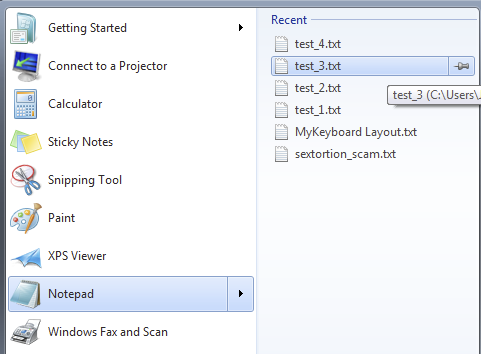
\includegraphics[scale=.3]{images/jl.png}
        \item Rotate or Pin
	\item \scriptsize{\texttt{AppData/Roaming/Microsoft/Windows/Recent/AutomaticDestinations}}
        \item[]
    \end{itemize}
\end{frame}


\begin{frame}[fragile]
  \frametitle{3.6 Jump Lists}
    \begin{itemize}
        \item Jump List file names start with 16 hex characters
	\item File names end with \texttt{.automaticDextinations-ms}
	\item[]
  \begin{lstlisting}[basicstyle=\tiny]
C:> dir \Users\John\AppData\Roaming\Microsoft\Windows\Recent\AutomaticDestinations

04/05/2020  12:50            33 792 1b4dd67f29cb1962.automaticDextinations-ms
14/06/2019  16:43             4 608 28c8b86deab549a1.automaticDextinations-ms
10/04/2019  14:32            29 696 6824f4a902c78fbd.automaticDextinations-ms
10/04/2020  14:12             9 216 7e4dca80246863e3.automaticDextinations-ms
04/05/2020  12:50             8 704 918e0ecb43d17e23.automaticDextinations-ms
10/04/2019  14:30             3 072 b74736c2bd8cc8a5.automaticDextinations-ms
09/04/2019  14:43             6 144 de48a32edcbe79e4.automaticDextinations-ms
  \end{lstlisting}
	\item Each Hex value correspond to an application
	\item \texttt{918e0ecb43d17e23 = Notepad.exe}
	\item Hex values are fixed world wide
        \item Search for Jump List IDs
    \end{itemize}
\end{frame}


\begin{frame}[fragile]
  \frametitle{3.6 Jump Lists}
    \begin{itemize}
        \item Exercise: Identify applications
  \begin{lstlisting}[basicstyle=\tiny]
$ cd JumpLists/AutomaticDestinations/
$ ll

    1b4dd67f29cb1962.automaticDestinations-ms --> 
    28c8b86deab549a1.automaticDestinations-ms --> 
    6824f4a902c78fbd.automaticDestinations-ms --> 
    7e4dca80246863e3.automaticDestinations-ms --> 
    918e0ecb43d17e23.automaticDestinations-ms --> 
    b74736c2bd8cc8a5.automaticDestinations-ms --> 
    de48a32edcbe79e4.automaticDestinations-ms --> 
  \end{lstlisting}
	\item Exercise: Analyze the Notepad Jump List file
  \begin{lstlisting}[basicstyle=\tiny]










-
  \end{lstlisting}
    \end{itemize}
\end{frame}


\begin{frame}[fragile]
  \frametitle{3.6 Jump Lists}
    \begin{itemize}
        \item Exercise: Identify applications
  \begin{lstlisting}[basicstyle=\tiny]
$ cd JumpLists/AutomaticDestinations/
$ ll

    1b4dd67f29cb1962.automaticDestinations-ms --> Windows Explorer
    28c8b86deab549a1.automaticDestinations-ms --> Internet Explorer 8
    6824f4a902c78fbd.automaticDestinations-ms --> Firefox 64.x
    7e4dca80246863e3.automaticDestinations-ms --> Control Panel
    918e0ecb43d17e23.automaticDestinations-ms --> Notepad (32-bit)
    b74736c2bd8cc8a5.automaticDestinations-ms --> WinZip
    de48a32edcbe79e4.automaticDestinations-ms --> Acrobat Reader 15.x
  \end{lstlisting}
	\item Exercise: Analyze the Notepad Jump List file
  \begin{lstlisting}[basicstyle=\tiny]










-
  \end{lstlisting}
    \end{itemize}
\end{frame}


\begin{frame}[fragile]
  \frametitle{3.6 Jump Lists}
    \begin{itemize}
        \item Exercise: Identify applications
  \begin{lstlisting}[basicstyle=\tiny]
$ cd JumpLists/AutomaticDestinations/
$ ll

    1b4dd67f29cb1962.automaticDestinations-ms --> Windows Explorer
    28c8b86deab549a1.automaticDestinations-ms --> Internet Explorer 8
    6824f4a902c78fbd.automaticDestinations-ms --> Firefox 64.x
    7e4dca80246863e3.automaticDestinations-ms --> Control Panel
    918e0ecb43d17e23.automaticDestinations-ms --> Notepad (32-bit)
    b74736c2bd8cc8a5.automaticDestinations-ms --> WinZip
    de48a32edcbe79e4.automaticDestinations-ms --> Acrobat Reader 15.x
  \end{lstlisting}
	\item Exercise: Analyze the Notepad Jump List file
  \begin{lstlisting}[basicstyle=\tiny]
$ 7z l 918e0ecb43d17e23.automaticDestinations-ms
        Date      Time    Attr         Size   Compressed  Name
     ------------------- ----- ------------ ------------  -------
                         .....         1398         1408  2
                         .....         1368         1408  1
                         .....          436          448  4
                         .....          392          448  3

--> file
--> exiftool
--> strings              --> $ strings -el DestList
  \end{lstlisting}
    \end{itemize}
\end{frame}




